\section{Introduction}
Processing large volumes of data in batch is often not sufficient in cases where new data has to be processed fast to quickly adapt and react to changes. For that reason, stream data processing (SDP) has gained significant attention. The most popular engines used for SDP, with large-scale adoption by industry and the research community, are Apache Storm \cite{toshniwal2014storm}, Apache Spark  \cite{zaharia2012discretized}, and Apache Flink \cite{carbone2015apache}. 

\begin{figure*}
    \centering
    \begin{subfigure}[b]{0.3\textwidth}
        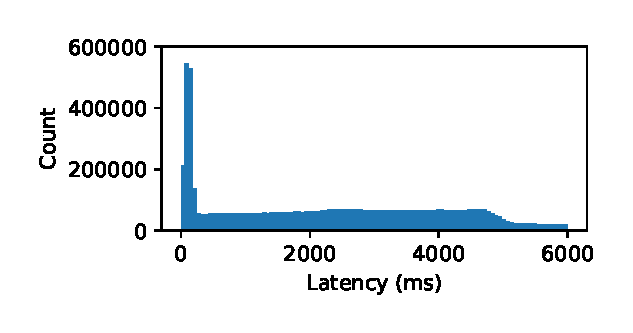
\includegraphics[width=\textwidth]{2nodesize2_hist}

        \caption{Storm, 2-node, max  throughput }
    \end{subfigure}
    ~ 
    \begin{subfigure}[b]{0.3\textwidth}
        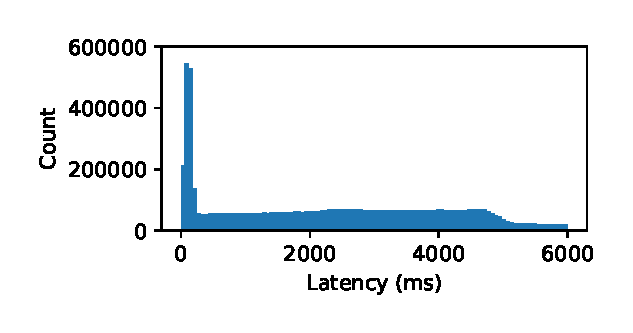
\includegraphics[width=\textwidth]{2nodesize2_hist}

        \caption{Storm, 4-node, max   throughput }
    \end{subfigure}
    ~ 
    \begin{subfigure}[b]{0.3\textwidth}
        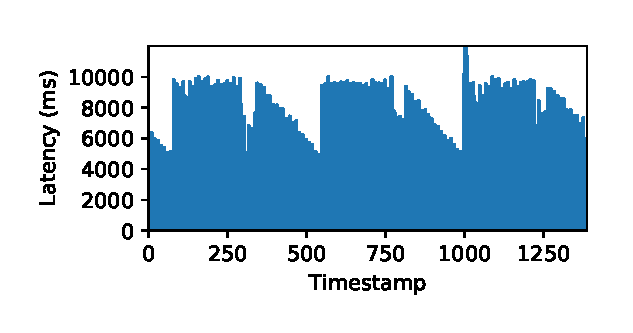
\includegraphics[width=\textwidth]{2nodesize2_ts}

        \caption{Storm, 8-node, max  throughput }
        
    \end{subfigure}
\end{figure*}

One  important application area of SDP is  online video games. These require the fast processing  of large scale online data feeds  from different sources. Windowed aggregations and windowed joins are two main operations that are used to monitor user feeds. One typical use-case is tracking the in-application-purchases (IAPs) per application, per distribution channel, or per product item (in-app products). Another typical use-case is the monitoring of advertising:  making sure that all campaigns and advertisement networks work flawlessly. Yet another use-case is comparing different user feeds by  joining them. For example, monitoring the IAPs of the same game downloaded from different distribution channels and comparing users'  actions  are essential in  online video game monitoring.


% \todo[inline]{Try to reflect Henri's comments: I suggest to first describe the jobs generically, i.e., aggregations and joins, and then relate them to the online game use cases of Rovio that Henri described (both what they do and what they plan to do).=>fixed}

In this work, we propose a benchmarking framework to accurately measure the performance of stream data processing engines. For our experimental evaluation, we test three publicly available open source and community driven engines, namely Apache Storm, Apache Spark, and Apache Flink.  
We measure the latency and throughput as the major performance indicators. Latency, in SDP, is the time difference between data production at the source (e.g., the mobile device) to result output at the sink of the data flow graph describing the stream processing operations (e.g., the monitoring solution on the game server). Throughput, in this scenario, determines the number of ingested and successfully processed records or events per time unit.

%In this paper we inspired from the quote of Napoleon Bonaparte being "Ability is nothing without opportunity". 
%Giving opportunity to all systems to express their ability is the key in benchmarking. 
Even though there have been several comparisons of the performance of SDPS recently, these do not measure the latencies and throughput that can be achieved in a production setting. One of the repeating problems in the previous evaluations is a missing definition and inaccurate measurement procedure for latency of stateful operators in SDPS. Another challenge is a missing separation between the system under test (SUT) and the benchmark driver. Frequently, the performance metrics are measured and calculated within SUT; this means that the results will be influenced through the measurements and, thus, can be biased. %Another challenge is, enabling the driver to be flexible enough to support different policies to handle system specific features. For example, back-pressure is characteristic feature of SDPSs and while calculating a system's sustainability with a given workload, it must be taken into consideration. Most importantly, it is essential to  keep the benchmarking system simple while solving the challenges listed above
We discuss in detail these challenges as well as our solutions in Section \ref{chal}.


% For example, there are numerous open challenges related with measuring main Key Performance Indicators (KPIs) in stream data processing engines. One of them is lacking the clear definition for the latency of stateful operator in SDPS.   The stream and its output are theoretically infinite and, therefore, the methods to measure its latency  have to be different from the batch processing systems. While the some works \cite{chintapalli2016benchmarking}, checkpoint events' timestamps in another system, this can  escalate the driver's complexity and create \textit{artificial latency}. Although the authors define latency as an average time span from the arrival of record till the end of its processing \cite{lu2014stream}, this definition is optimistic. In real life scenarios, the actual latency is calculated from the event's generation time. Moreover, when benchmarking SDPSs, it is crucial to separate the driver and system under test completely as otherwise, the results can be biased \todo[inline]{why?}. Furthermore, the driver should be flexible enough to support different policies to handle system specific features. For example, back-pressure is characteristic feature of SDPSs and while calculating a system's sustainability with a given workload, it must be taken into consideration.
%Most importantly, it is essential to  keep the benchmarking system simple while solving the challenges listed above. 

In this paper, we address the above mentioned challenges. The proposed solution is generic, has a clean design with clear semantics, and can be applied to any SDPS. The main goal is to stimulate an environment in which we can measure the metrics more precisely and with minimum influence of side factors.

The main contributions of this paper go as follows:
\begin{itemize}  
\item We    introduce a mechanism to accurately measure the latency of stateful operators in SDPSs. We apply the proposed method to use-cases featuring windowed aggregations and windowed joins. 
\item We accomplish the complete separation of the test driver from the system under test (SUT). 
 %\todo[inline]{the second sentence is unclear=>deleted}
\item We measure the maximum sustainable throughputs of the SDPSs. Our benchmarking framework handles system specific features like backpressure to measure the maximum sustainable throughput of a system. 
%\item We accomplish the above contributions with a simple system design with minimum components being System Under Test (SUT) and Data Engine. 
\item We use the proposed benchmarking system for an extensive evaluation of Storm, Spark, and Flink with practical use-cases.
\end{itemize}

The remainder of this paper is organized as follows. In Section \ref{rel}, we survey the related work. We give an overview of the stream data processing engines benchmarked in this paper in Section \ref{pre}. In Section \ref{chal}, we discuss the detailed interpretation of stream benchmarking challenges and their importance. We provide the design of our benchmarking system, the use-cases, and the metrics in Section \ref{des}. After a detailed evaluation in Section \ref{eval}, we conclude in Section \ref{conc}.
